% Git Leak Hunter -- project report in IEEE conference format (IEEEtran).
% Build: cd docs/report && pdflatex ieee-report.tex && pdflatex ieee-report.tex
%
% Every number in this document comes from a run that actually happened: the committed benchmark
% results (bench/results/*.json, docs/BENCHMARK.md, docs/RULES.md) or the commands listed in
% Section VII, run on the machine and date stated there.
\documentclass[conference]{IEEEtran}
\IEEEoverridecommandlockouts

\usepackage[T1]{fontenc}
\usepackage{lmodern}
\usepackage{microtype}
\DisableLigatures[-]{encoding=T1,family=tt*}
\usepackage{cite}
\usepackage{amsmath,amssymb}
\usepackage{graphicx}
\usepackage{booktabs}
\usepackage{multirow}
\usepackage{array}
\usepackage{xcolor}
\usepackage{tikz}
\usetikzlibrary{arrows.meta,positioning,fit,shapes.misc}
\usepackage{pgfplots}
\pgfplotsset{compat=1.18}
\usepackage{listings}
\usepackage{url}
\usepackage[hidelinks]{hyperref}

\lstset{basicstyle=\ttfamily\scriptsize,columns=fullflexible,keepspaces=true,
  breaklines=true,frame=single,framesep=2pt,xleftmargin=3pt,xrightmargin=3pt}

\makeatletter
\newcommand{\linebreakand}{\end{@IEEEauthorhalign}\hfill\mbox{}\par\mbox{}\hfill\begin{@IEEEauthorhalign}}
\makeatother

\newcommand{\tool}{Git Leak Hunter}
\newcommand{\code}[1]{\texttt{#1}}
\newcolumntype{P}[1]{>{\raggedright\arraybackslash}p{#1}}
\newcommand{\hd}[1]{\begin{tabular}[b]{@{}c@{}}#1\end{tabular}}

\begin{document}

\title{Git Leak Hunter: A Defensive Full-History Secret-Exposure Scanner for Git Repositories and CI/CD Configuration}

\author{
\IEEEauthorblockN{Pruthvi Gangapure}
\IEEEauthorblockA{Roll No. 12415034}
\and
\IEEEauthorblockN{Prathamesh Yewale}
\IEEEauthorblockA{Roll No. 12413969}
\and
\IEEEauthorblockN{Yash Waghmare}
\IEEEauthorblockA{Roll No. 12410801}
\and
\IEEEauthorblockN{Chetan Thakur}
\IEEEauthorblockA{Roll No. 12413081}
\linebreakand
\IEEEauthorblockN{Guide: Prof.\ Jyoti Yadav}
\IEEEauthorblockA{Ethical Hacking Course Project, Group 34}
}

\maketitle

\begin{abstract}
Credentials committed to a Git repository remain recoverable from its history even after a later
commit deletes them, and CI/CD configuration files are a frequent, under-scanned place for such
literals. This report presents \tool{}, a defensive command-line scanner that walks the
\emph{entire reachable history} of a repository, detects secrets with a hybrid of vendor-specific
signatures and length-normalised Shannon entropy, parses GitHub Actions, GitLab CI and Dockerfile
configuration structurally, classifies every finding with a table-driven severity function, and
reports whether each secret is still present at \code{HEAD} or exists only in history. Detection
results are memoised by blob hash, so the work done is proportional to the number of unique blobs
rather than to commits~$\times$~files. Optional live verification is opt-in, read-only, and limited
to two allowlisted endpoints. No output ever contains a full secret. The implementation consists of
4{,}545 lines of TypeScript with a 306-test suite. On the project's eight synthetic fixture
repositories (32 planted fabricated secrets) it reported all 32 with no false positives, against
28 for Gitleaks~8.30.1 and 14 for TruffleHog~3.99.3 in their default configurations; we discuss
why this home-field result does not measure real-world accuracy. On a synthetic history with high
blob reuse, memoisation reduced the median scan time of a 4{,}000-commit repository from
1084~ms to 164~ms.
\end{abstract}

\begin{IEEEkeywords}
secret detection, credential leakage, Git history, software supply chain, CI/CD security,
Shannon entropy, memoization, ethical hacking
\end{IEEEkeywords}

% ---------------------------------------------------------------------------------------------
\section{Introduction}

Hard-coded credentials (CWE-798~\cite{cwe798}) are one of the most common ways that cloud
accounts, package registries and CI/CD systems are compromised. Large-scale measurement shows that
secret leakage in public repositories is widespread and that leaked keys are often not
removed~\cite{meli2019}. The usual remediation, deleting the secret in a new commit, does not help:
Git is a content-addressed object store, and every earlier version of every file remains reachable
from the commit graph until history is rewritten~\cite{filterrepo}. A scanner that inspects only
the working tree therefore misses exactly the secrets a developer believes are gone.

CI/CD pipelines widen the problem. Workflow files, pipeline variables and container build
arguments routinely carry tokens, and insufficient credential hygiene is listed among the top
CI/CD security risks~\cite{owaspcicd}. Compromise of a single CI credential can cascade through
the software supply chain, as the 2021 Codecov Bash-uploader incident demonstrated~\cite{codecov}.

\tool{} is a defensive tool built for repository owners. Given a local path or a remote URL, it
answers four questions for every committed secret: \emph{what} it is, \emph{where} and in
\emph{which commit} it was introduced, \emph{how severe} the exposure is, and \emph{whether it is
still present} at \code{HEAD} or recoverable only from history.

\subsection{Contributions}
\begin{itemize}
\item A four-stage pipeline (\textsc{Detect} $\rightarrow$ \textsc{Analyze} $\rightarrow$
  \textsc{Verify} $\rightarrow$ \textsc{Report}) that walks every commit on every ref, including
  each parent side of merge commits, and reads content by blob hash without checking anything out.
\item Blob-hash memoisation that reduces detection work from $O(\text{commits}\times\text{files})$
  to $O(\text{unique blobs})$, verified by a reachable-blob invariant test.
\item A hybrid detector combining nine signature rules with a length-normalised entropy threshold,
  thirteen counted suppression reasons, and structural parsers for GitHub Actions, GitLab CI,
  Dockerfiles and eight kinds of credential file.
\item A safety design in which no data structure that reaches an output carries a raw secret,
  enforced by a JSON schema with \code{additionalProperties: false} and leak tests over every
  output channel.
\item Hardening for the fact that the scanned repository is untrusted input: no hooks, no
  submodule recursion, NUL-delimited parsing, ReDoS-bounded detectors, and an XSS-safe report.
\item A reproducible evaluation against Gitleaks~\cite{gitleaks} and TruffleHog~\cite{trufflehog}
  with an explicit list of the comparison's limitations.
\end{itemize}

The rest of this report is organised as follows. Section~\ref{sec:related} reviews related work.
Section~\ref{sec:threat} states the threat model and design rules. Sections~\ref{sec:arch}
and~\ref{sec:hardening} describe the architecture and its hardening. Section~\ref{sec:impl} covers
the implementation, Section~\ref{sec:eval} the evaluation, Section~\ref{sec:limits} limitations,
and Section~\ref{sec:ethics} responsible use.

% ---------------------------------------------------------------------------------------------
\section{Background and Related Work}\label{sec:related}

\subsection{Secret leakage in source repositories}
Meli \emph{et al.}~\cite{meli2019} scanned public GitHub at scale and found that leaked API keys and
private keys are common, that many remain in place, and that leaks appear in history as well as in
the current tree. Sinha \emph{et al.}~\cite{sinha2015} studied the detection and mitigation of
API-key leaks in source repositories. Basak \emph{et al.} released SecretBench~\cite{secretbench},
a labelled dataset of software secrets for evaluating detectors, and surveyed practitioner
practices for secret management~\cite{basak2022}. These studies motivate two design choices of
\tool{}: scanning full history and treating detector precision as a first-class concern.

\subsection{Existing scanners}
Gitleaks~\cite{gitleaks} is a regex-based scanner for Git repositories, files and standard input.
TruffleHog~\cite{trufflehog} combines a large detector library with optional live verification.
GitHub secret scanning~\cite{ghsecretscanning} runs provider-defined patterns on hosted
repositories. \tool{} differs in emphasis rather than in kind: it (i)~parses CI/CD files
structurally instead of as plain text, (ii)~reports \emph{presence} (in-\code{HEAD} versus
history-only) for every finding, (iii)~diffs merge commits against every parent so that secrets
introduced only during conflict resolution are found, and (iv)~is built so that a full secret
cannot reach any output.

\subsection{Shannon entropy}
For a string $X$ over an alphabet with empirical symbol frequencies $p(x_i)$, Shannon
entropy~\cite{shannon1948} in bits per character is
\begin{equation}
H(X) = -\sum_i p(x_i)\,\log_2 p(x_i).
\label{eq:entropy}
\end{equation}
Randomly generated tokens have higher $H$ than identifiers and prose, which makes $H$ a common
second-stage filter for candidates that no vendor signature recognises.

% ---------------------------------------------------------------------------------------------
\section{Threat Model and Design Rules}\label{sec:threat}

\subsection{Assets and adversaries}
The asset is any credential committed to a repository the user owns or is authorised to assess.
The tool must withstand two adversaries. The first is an outside attacker who mines public
history for credentials; the tool's purpose is to find those credentials first. The second is the
\emph{scanned repository itself}: file names, paths, commit messages, author names, Git
configuration and file contents are attacker-controlled input that may try to execute code,
inject Git options, forge parser boundaries, exhaust resources, or inject script into the HTML
report.

\subsection{Design rules}
The project's working rules (\code{CLAUDE.md}) translate into six binding requirements:
\begin{enumerate}
\item[R1] \textbf{No full secret in any output}: HTML, JSON, console, logs, errors or test output.
\item[R2] \textbf{No fabricated numbers}: every reported figure comes from a script that ran, with
  tool versions, commands, machine and date recorded.
\item[R3] \textbf{Verification is opt-in, read-only and allowlisted}: it needs both
  \code{--verify} and \code{--confirm-authorized}, and only \code{sts.amazonaws.com} and
  \code{api.github.com} may be contacted.
\item[R4] \textbf{Fabricated fixtures only}: test secrets are generated at test time from
  fragments, and no token-shaped literal is ever committed.
\item[R5] \textbf{Scanned repositories are untrusted}: Git is spawned with an argument vector,
  never a shell string; hooks are disabled and nothing from the target is executed.
\item[R6] \textbf{No feature creep}: features beyond the specification require approval.
\end{enumerate}

\subsection{Non-goals}
The tool does not exploit, enumerate or store discovered credentials, does not rewrite history,
and does not scan repositories the user is not authorised to scan.

% ---------------------------------------------------------------------------------------------
\section{System Architecture}\label{sec:arch}

Fig.~\ref{fig:pipeline} shows the pipeline, and Table~\ref{tab:model} the data model
\code{Repository} $\rightarrow$ \code{ContentUnit} $\rightarrow$ \code{Finding} $\rightarrow$
\code{Report}.

\begin{figure}[t]
\centering
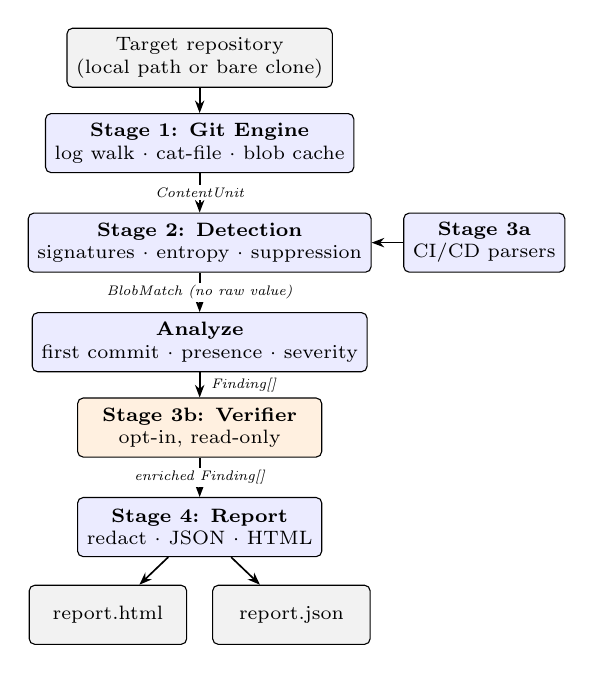
\begin{tikzpicture}[
  node distance=3.2mm,
  box/.style={draw,rounded corners=2pt,align=center,font=\scriptsize,minimum width=31mm,
    minimum height=7.5mm,fill=#1},
  box/.default=white,
  arr/.style={-{Stealth[length=1.6mm]},semithick},
  lab/.style={font=\tiny\itshape,fill=white,inner sep=1pt}]
\node[box=gray!10] (t) {Target repository\\(local path or bare clone)};
\node[box=blue!8,below=of t] (g) {\textbf{Stage 1: Git Engine}\\log walk $\cdot$ cat-file $\cdot$ blob cache};
\node[box=blue!8,below=5mm of g] (d) {\textbf{Stage 2: Detection}\\signatures $\cdot$ entropy $\cdot$ suppression};
\node[box=blue!8,right=4mm of d,minimum width=20mm] (ci) {\textbf{Stage 3a}\\CI/CD parsers};
\node[box=blue!8,below=5mm of d] (a) {\textbf{Analyze}\\first commit $\cdot$ presence $\cdot$ severity};
\node[box=orange!12,below=of a] (v) {\textbf{Stage 3b: Verifier}\\opt-in, read-only};
\node[box=blue!8,below=5mm of v] (r) {\textbf{Stage 4: Report}\\redact $\cdot$ JSON $\cdot$ HTML};
\node[box=gray!10,below left=3.5mm and -14mm of r,minimum width=20mm] (h) {report.html};
\node[box=gray!10,below right=3.5mm and -14mm of r,minimum width=20mm] (j) {report.json};
\draw[arr] (t) -- (g);
\draw[arr] (g) -- node[lab]{ContentUnit} (d);
\draw[arr] (ci) -- (d);
\draw[arr] (d) -- node[lab]{BlobMatch (no raw value)} (a);
\draw[arr] (a) -- node[lab,right=1mm]{Finding[]} (v);
\draw[arr] (v) -- node[lab]{enriched Finding[]} (r);
\draw[arr] (r) -- (h);
\draw[arr] (r) -- (j);
\end{tikzpicture}
\caption{The \textsc{Detect}$\rightarrow$\textsc{Analyze}$\rightarrow$\textsc{Verify}$\rightarrow$\textsc{Report}
pipeline. Raw secret values never cross the Detection$\rightarrow$Analyze boundary.}
\label{fig:pipeline}
\end{figure}

\begin{table}[t]
\centering
\caption{Data Model (\code{src/types.ts})}
\label{tab:model}
\footnotesize
\begin{tabular}{@{}P{17mm}P{63mm}@{}}
\toprule
Type & Meaning \\
\midrule
\code{ContentUnit} & One file version as seen in one commit: repository, commit hash, author,
  date, path, blob hash, content, origin (\code{history}/\code{head}), line offsets. \\
\code{Finding} & One secret at one location: location-based fingerprint, rule, detector,
  severity, path, commit, line, column, \emph{redacted} preview and context, entropy,
  first-seen commit, other-commit count, presence, verification status. \textbf{No raw-secret
  field.} \\
\code{Report} & Repository, scan options, measured statistics, severity summary and sorted
  findings; serialised as \code{report.json} and rendered as \code{report.html}. \\
\bottomrule
\end{tabular}
\end{table}

\subsection{Stage 1: Git engine}
The engine opens a local repository, or bare-clones a remote URL into a temporary directory with
an empty template directory (so no hooks are installed) and no checkout. It then streams
\begin{quote}\footnotesize
\code{git log --topo-order --reverse -m --root --raw -z --no-abbrev --no-renames --no-ext-diff
--no-textconv --all}
\end{quote}
which yields, for every commit, its metadata and the list of changed paths with their new blob
hashes~\cite{gitlog}. The \code{-m} flag diffs each merge commit against \emph{each} parent, so a
secret introduced only while resolving a conflict is still seen. Content is read by blob hash
through a single long-lived \code{git cat-file --batch-command} process~\cite{gitcatfile}, which is
first asked for object \code{info} so that oversize blobs are never transferred. No commit is ever
checked out.

\emph{Streaming parser.} Output is split into NUL-terminated tokens as it arrives. Each commit
header begins with a marker that carries a random per-run nonce, so an attacker-chosen commit
subject or file name cannot forge a commit boundary. Memory therefore grows with the number of file
versions, not with blob content.

\emph{Memoisation.} A naive scanner reads every file of every commit, i.e.\
$O(\text{commits}\times\text{files})$ work. \tool{} reads only the files each commit changed and
caches detection results under the key
\begin{equation}
k = \textit{configHash} \,\|\, \textit{blobHash} \,\|\, \textit{fileKind},
\end{equation}
so identical content reached through other commits, paths, branches or reverts is scanned once,
giving $O(\text{unique blobs})$ detection work~\cite{clrs}. The file kind is part of the key
because the same bytes are parsed differently as a workflow file and as documentation. Severity
depends on path class and presence, so it is applied after the cache. Tests assert that the
scanner function runs exactly once per unique (blob, kind) and that
\begin{equation}
\textit{uniqueBlobsScanned} + \textit{cacheHits} = \textit{fileVersionsSeen}.
\end{equation}

\emph{Reachable-blob invariant.} For every fixture repository, with and without ignore rules, a test
checks that
\begin{equation}
S_{\text{scanned}} \cup S_{\text{skipped}} \cup S_{\text{ignored}} = S_{\text{rev-list}},
\end{equation}
where $S_{\text{rev-list}}$ is the set of blobs listed by \code{git rev-list --objects --all}. The
test fails if any commit-reachable blob, including one that exists only in a merge resolution, was
never considered.

\emph{Presence.} After the walk, the \code{HEAD} tree (or the \code{--branch} tip) is listed. A
finding is \code{in-HEAD} if the same secret is found at the same path there, and
\code{history-only} otherwise.

\subsection{Stage 2: Detection engine}
\subsubsection{Candidate generation}
Candidates come from three sources: vendor signatures (Table~\ref{tab:signatures}), structured
parsing of CI/CD and credential files (Section~\ref{sec:ci}), and generic \code{key = value}
assignments whose key name looks secret-like (\code{api\_key}, \code{secret}, \code{token},
\code{password}, \ldots). Overlapping spans are resolved by priority
signature $>$ credential file $>$ CI $>$ entropy.

\begin{table}[t]
\centering
\caption{Signature Rules (\code{src/detect/signatures.ts})}
\label{tab:signatures}
\footnotesize
\begin{tabular}{@{}P{24mm}P{56mm}@{}}
\toprule
Rule & Pattern (summary) \\
\midrule
AWS access key ID & \code{AKIA}/\code{ASIA}/\code{AIDA} + 16 \code{[A-Z0-9]}, not inside a longer token \\
AWS secret key & 40 chars \code{[A-Za-z0-9/+]} within 5 lines of a key ID, not all-hex, must pass entropy \\
GitHub token & \code{ghp\_ gho\_ ghu\_ ghs\_ ghr\_} + 36 alphanumerics \\
GitHub fine-grained & \code{github\_pat\_} + 22 + \code{\_} + 59 alphanumerics \\
Stripe live / test & \code{sk\_live\_}/\code{rk\_live\_}, \code{sk\_test\_}/\code{rk\_test\_} + $\geq$16 alphanumerics \\
Slack token & \code{xox[abprs]-} + dash-separated segments \\
Slack webhook & \code{https://hooks.slack.com/services/\ldots} \\
Private key & PEM \code{BEGIN \ldots{} PRIVATE KEY} header through the matching footer (or 200 lines) \\
\bottomrule
\end{tabular}
\end{table}

Each AWS key ID is paired with the nearest unclaimed 40-character candidate within five lines;
both findings record each other's fingerprint, which is what live verification needs. A
private-key block is one finding at its header line, with a preview such as
``\code{BEGIN RSA PRIVATE KEY [REDACTED, 14 lines]}''; the PEM dashes are dropped deliberately so
that a report never looks like a key file to another scanner.

\subsubsection{Length-normalised entropy}
A string of length $n$ cannot exceed $\log_2 n$ bits per character, and random strings measure
well below that bound. A fixed 4.5-bit threshold for base64-like strings is therefore unreachable
for 20--22-character strings and rejects most random 24--32-character secrets
(Table~\ref{tab:entropy}). \tool{} classifies each candidate's charset as hex, base64-like or
other, with alphabet size $A\in\{16,64,94\}$, and uses the effective threshold
\begin{equation}
T_{\text{eff}} = \min\!\Big(T_{\text{charset}},\; \lambda \log_2 \min\big(\max(n, n_{\min}),\, A\big)\Big)
\label{eq:teff}
\end{equation}
with $\lambda = 0.85$, defaults $T_{\text{hex}}=3.0$, $T_{\text{base64}}=4.5$ and $n_{\min}=20$.
Long strings are held to the configured threshold, and shorter strings must reach 85\% of the
maximum entropy a string of that length could have. Normalising at $\max(n,n_{\min})$ rather than
$n$ prevents short words from passing: \code{postgres1} (9 characters) has $H=2.948$, above
$0.85\log_2 9 = 2.69$, but below the threshold for a 20-character string.

\subsubsection{False-positive suppression}
Thirteen suppression reasons are implemented and each dropped candidate increments a counter in
the report: inline \code{leakhunter:ignore}, documentation example keys, repeated characters,
placeholders (\code{changeme}, \code{your\_api\_key\_here}, \ldots), CI expressions
(\code{\$\{\{ \ldots{} \}\}}), environment references (\code{\$VAR}, \code{\$\{VAR\}},
\code{\%VAR\%}, \code{process.env.X}, \ldots), RFC~4122 UUIDs~\cite{rfc4122}, 40-hex Git SHAs,
lockfile integrity hashes, data URIs, vendored paths, low entropy, and fingerprints listed in an
ignore file. Signature matches are exempt from the UUID, SHA and lockfile rules, so a real token
inside a lockfile is still reported.

\subsection{Stage 3a: CI/CD and credential files}\label{sec:ci}
The file kind is derived from the path and is part of the cache key, so all of the following are
scanned across history, not only at \code{HEAD}:
\begin{itemize}
\item \textbf{GitHub Actions}: literal scalars under \code{env:} (workflow, job, step, container,
  services), \code{with:} inputs and container \code{credentials:}.
\item \textbf{GitLab CI}: global and job \code{variables:}, including \code{\{ value: \ldots{} \}}
  and \code{include: local} files.
\item \textbf{Dockerfile}: \code{ENV K=V}, legacy \code{ENV K V} and \code{ARG K=V}, with
  backslash continuations joined through an offset map.
\item \textbf{Credential files}: \code{.env}, \code{.npmrc}, \code{credentials*.json},
  \code{.docker/config.json}, SSH private-key files, \code{.pgpass}, \code{.netrc} and
  \code{.git-credentials}.
\end{itemize}
YAML is parsed into an AST so that source offsets give exact line and column. Malformed YAML
raises a parse error and the file is re-scanned as text, so a broken file never aborts a scan.
A literal under a secret-like key that fails the entropy check but is at least eight characters
long is reported as a \emph{weak} literal (Low).

\subsection{Analyze: attribution and severity}
\code{analyze.ts} groups matches into findings (one secret, one path, one rule), using a keyed HMAC
of the value with a per-run random key that is never written anywhere. It records the commit
that first introduced the secret at that path, how many other commits carried it, and presence.
The fingerprint is the first 32 hex characters of
$\mathrm{SHA\text{-}256}(\textit{ruleId}, \textit{blobHash}, \textit{path}, \textit{line},
\textit{column})$: it is location-based, stable across runs, and never derived from the secret.

Severity is a pure, table-driven function in which the first matching row wins
(Table~\ref{tab:severity}). Per-rule overrides may be set in a configuration file, but a
credential verified as active is always Critical.

\begin{table}[t]
\centering
\caption{Severity Table (\code{src/detect/severity.ts}); First Match Wins}
\label{tab:severity}
\footnotesize
\begin{tabular}{@{}c l P{48mm}@{}}
\toprule
\# & Severity & Condition \\
\midrule
1 & Critical & Live verification returned \code{ACTIVE} \\
2 & Critical & Private key still present at \code{HEAD} \\
3 & Critical & Stripe live key still present at \code{HEAD} \\
4 & Low & Secret-like key with a low-entropy literal \\
5 & High & Signature match for AWS, GitHub, Slack, live Stripe or a private key (incl.\ history-only) \\
6 & High & Literal secret in GitHub Actions, GitLab CI or a Dockerfile \\
7 & High & Committed credential file (\code{.env}, \code{.npmrc}, \code{id\_rsa}, \ldots) \\
8 & Medium & Stripe test key \\
9 & Low & Entropy-only candidate in tests, docs, examples or fixtures \\
10 & Medium & Entropy-only candidate in application code \\
11 & Low & Anything else \\
\bottomrule
\end{tabular}
\end{table}

\subsection{Stage 3b: Optional live verification}
Verification runs only when \emph{both} \code{--verify} and \code{--confirm-authorized} are given,
and an authorised-use banner is printed before any request. Exactly one read-only call is made per
unique credential:
\begin{itemize}
\item \textbf{AWS}: \code{POST https://sts.amazonaws.com/} with \code{Action=GetCallerIdentity}
  \cite{awssts}, signed with AWS Signature Version~4~\cite{awssigv4} using the paired key ID and
  secret. HTTP 200 means \code{ACTIVE}; \code{InvalidClientTokenId}, \code{SignatureDoesNotMatch},
  \code{ExpiredToken} or \code{AccessDenied} mean \code{INACTIVE}; anything else (including an
  unpaired key or temporary \code{ASIA} credentials) is \code{UNVERIFIABLE}.
\item \textbf{GitHub}: \code{GET https://api.github.com/user}~\cite{ghusers}; 200 is
  \code{ACTIVE}, 401 is \code{INACTIVE}, rate limiting and other outcomes are \code{UNVERIFIABLE}.
\end{itemize}
Guardrails: an exact-host, HTTPS-only allowlist checked before any request; no redirects; a 10~s
timeout; no retries; sequential calls 250~ms apart, at most 25 per provider; and a stop at the
first rate-limit response. The GitHub response body is never read, and from STS only the error
code is read, so no account identifiers are retained. SigV4 is implemented in about 60 lines rather
than by adding the AWS SDK and its dependency tree, and is tested against AWS's published signing
vectors.

When verification is on, raw values of verifiable rules are placed in an in-memory \emph{vault};
each match carries only an opaque random reference. The vault is cleared in a \code{finally} block
as soon as verification ends, and its \code{toJSON} prints only an entry count.

\subsection{Stage 4: Reporting and redaction}
\emph{Redaction.} Values of at least 12 characters are shown as the first 4 characters, 16 stars
and the last 4 (e.g.\ \code{AKIA****************WXYZ}); the star count is fixed so the preview does
not reveal the length. Shorter values show at most 2 leading characters and 8 stars. Context lines
are masked twice: first every detected span, then any residual token-like run of at least 16
characters that mixes letters and digits or is mixed-case with entropy $\geq 3.5$, so that an
undetected secret on the same line cannot leak. Commit subjects and author fields, which are
attacker-controlled and may contain pasted secrets, pass through the same masking.

\emph{JSON.} \code{report.json} is validated in the tests against a JSON Schema
(draft 2020-12~\cite{jsonschema}) that uses \code{additionalProperties: false} everywhere, so a
stray field, such as an accidentally added raw value, fails validation.

\emph{HTML.} \code{report.html} is a single self-contained file with inline CSS and one inline
script for filtering by severity and presence and for sorting. It loads no external resources and
sets the Content Security Policy~\cite{csp3}
\code{default-src 'none'; style-src 'unsafe-inline'; script-src 'unsafe-inline'}. Every dynamic
value is HTML-escaped and control characters in paths are shown as \code{\textbackslash xNN}.
Fig.~\ref{fig:report} shows a report generated from the \code{ci-configs} fixture.

\begin{figure}[t]
\centering
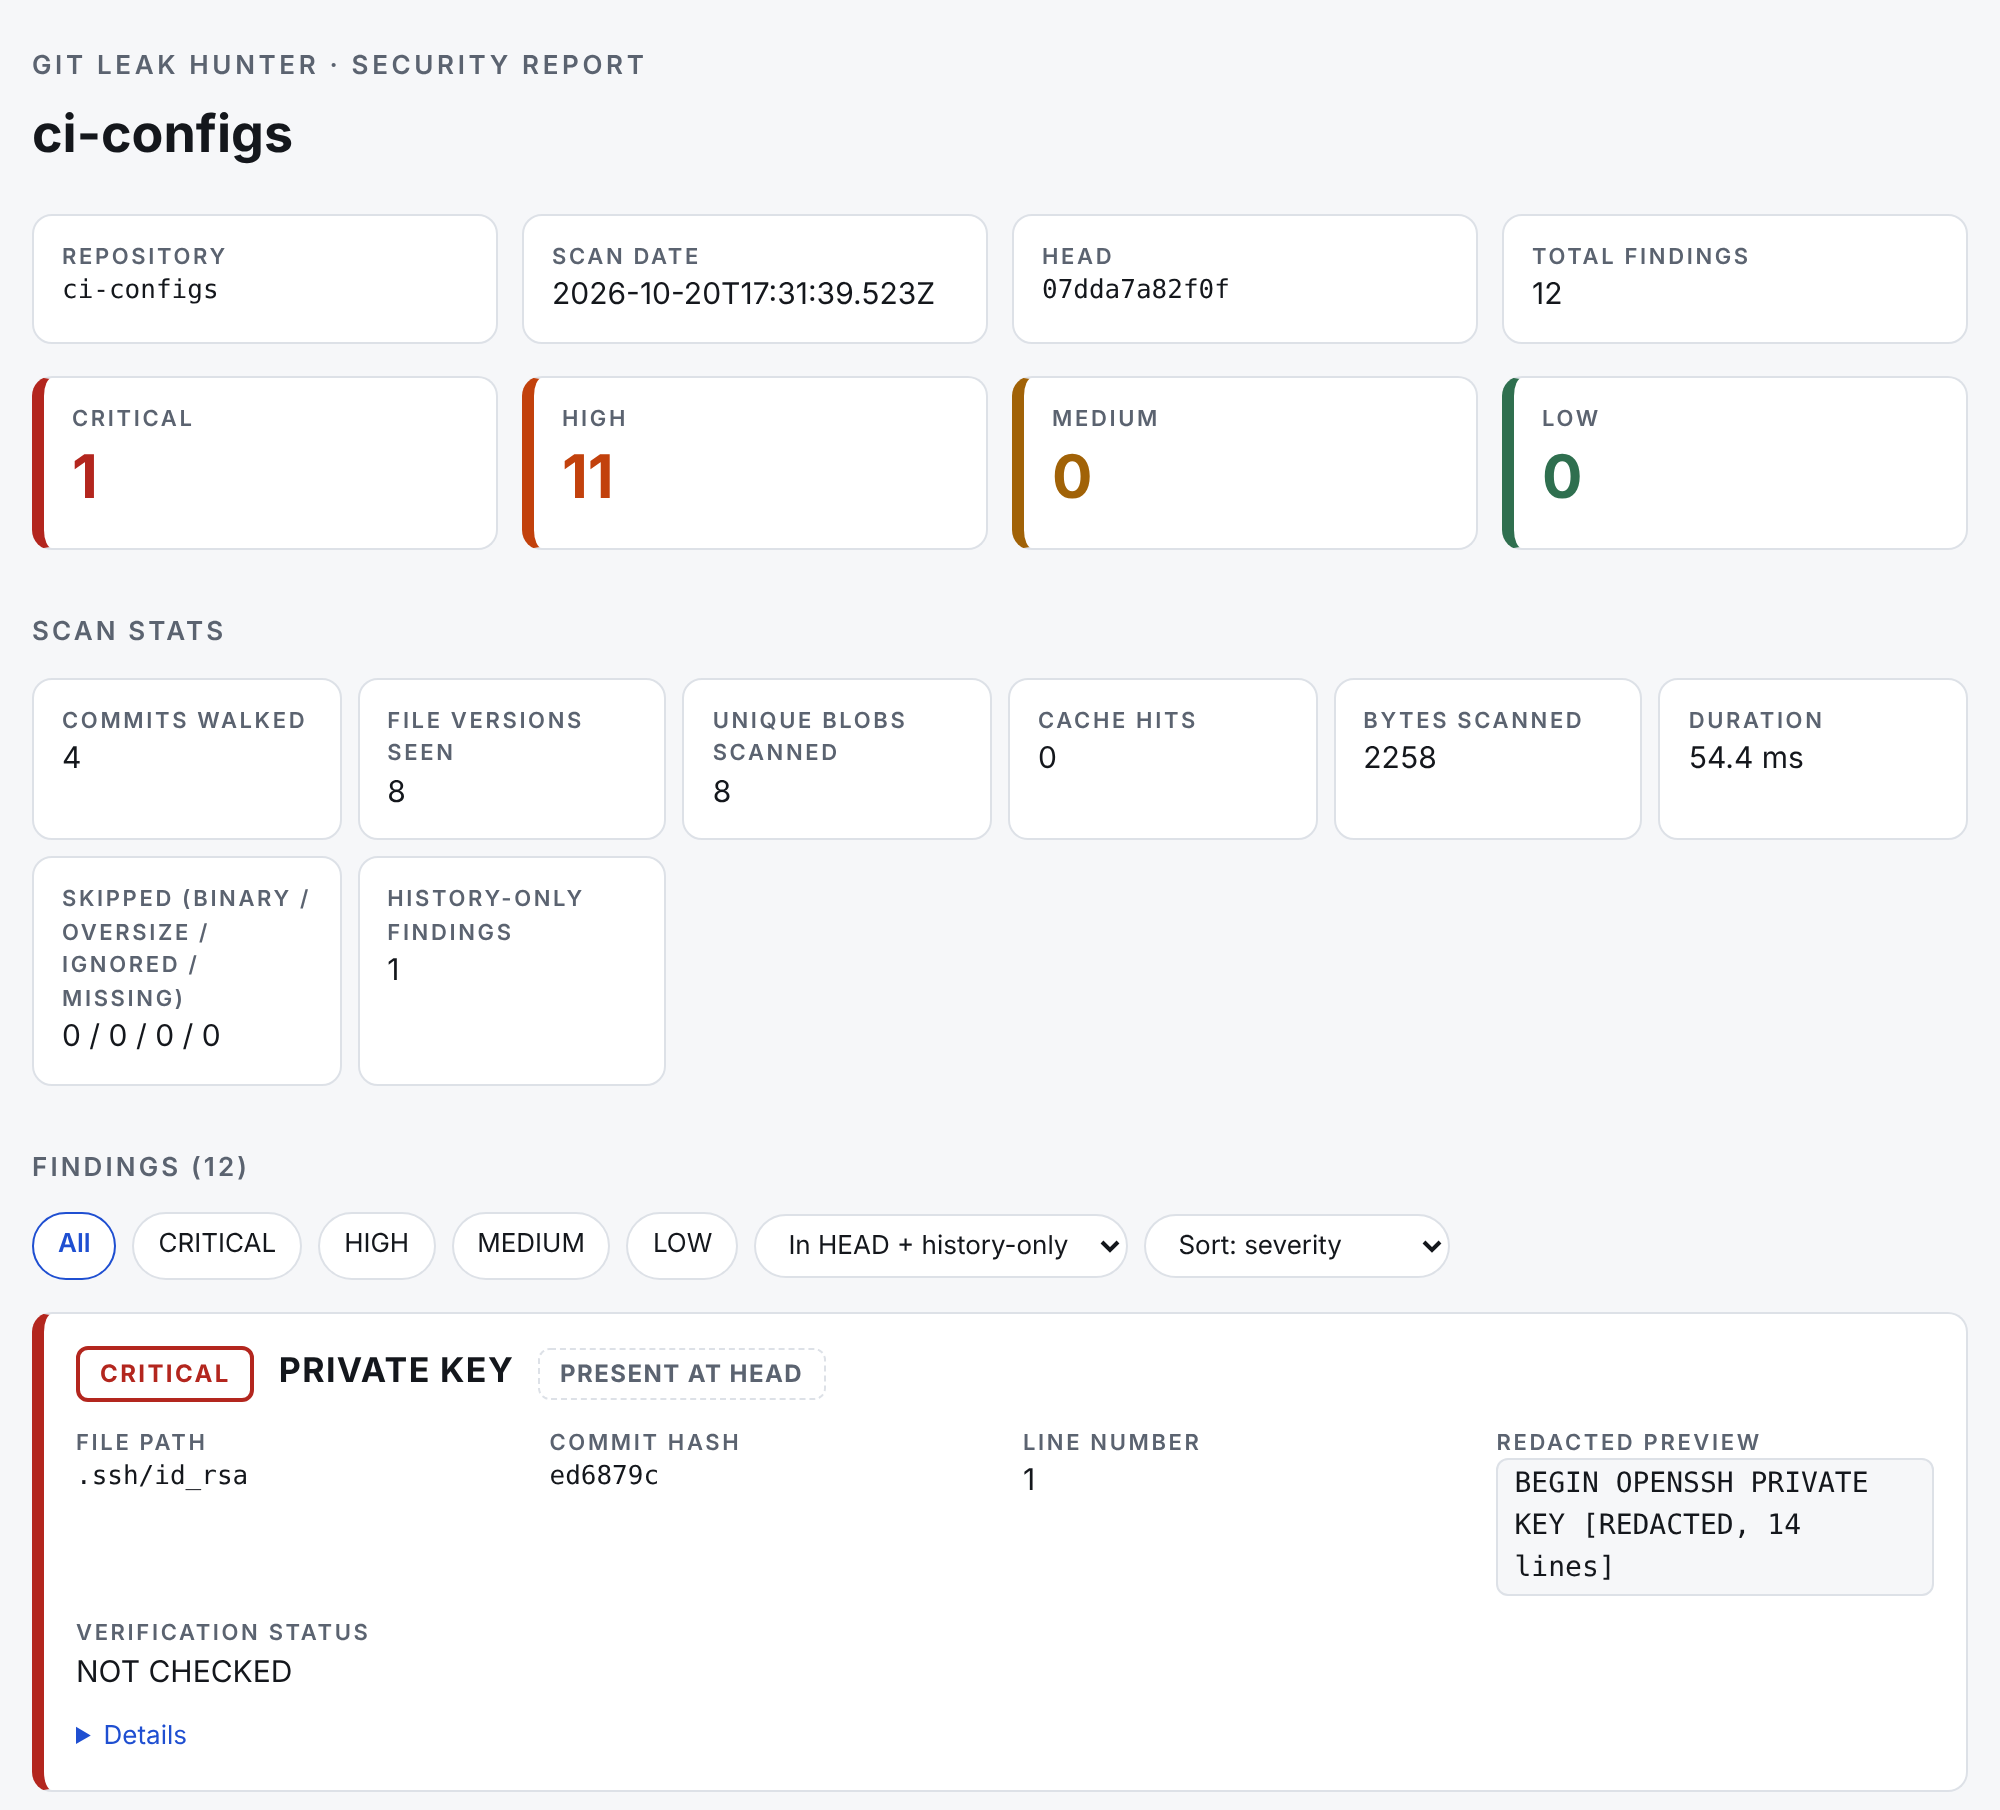
\includegraphics[width=\columnwidth]{figures/html-report.png}
\caption{Top of \code{examples/report.html}, generated from the \code{ci-configs} fixture
(fabricated secrets only). Severity counts, measured scan statistics and the first finding card
with its redacted preview and presence badge are visible.}
\label{fig:report}
\end{figure}

\subsection{Optional: owner-scoped GitHub dorking}
The \code{dork} sub-command runs built-in code-search terms (\code{AKIA}, \code{ghp\_},
\code{filename:.env}, \ldots) through the GitHub code-search API~\cite{ghsearch} and feeds the
matching files into the same detection and report pipeline. It is restricted to owners the user
controls: before any search the token's account must be the owner itself, or an active admin of
the organisation. Every query carries exactly one \code{user:}/\code{org:} qualifier added by the
tool, queries containing any other scope qualifier or \code{OR} are refused before the first
request, out-of-owner results are dropped, and requests are paced to the 10-per-minute search
budget, stopping at the first rate limit.

% ---------------------------------------------------------------------------------------------
\section{Hardening Against Untrusted Input}\label{sec:hardening}

Table~\ref{tab:hardening} summarises how the threats of Section~\ref{sec:threat} are mitigated and
which tests cover them. Every Git invocation goes through one module (\code{src/git/exec.ts}),
always with an argument vector, and is prefixed with
\begin{lstlisting}
-c core.hooksPath=/dev/null  -c core.fsmonitor=false
-c core.pager=cat            -c protocol.allow=never
-c protocol.https.allow=always
-c protocol.ssh.allow=always -c submodule.recurse=false
\end{lstlisting}
\noindent Variables
that would redirect Git (\code{GIT\_DIR}, \code{GIT\_WORK\_TREE}, \ldots) are removed from the
environment and terminal prompts are disabled.

\begin{table*}[t]
\centering
\caption{Threats From the Scanned Repository and Their Mitigations (\code{docs/ARCHITECTURE.md})}
\label{tab:hardening}
\footnotesize
\begin{tabular}{@{}P{48mm}P{80mm}P{32mm}@{}}
\toprule
Threat & Mitigation & Test \\
\midrule
Hooks, fsmonitor, pager, \code{ext::}/\code{file://} transports, submodules
  & \code{-c} overrides on every Git call; remote URL allowlist (\code{https}, \code{ssh})
  & \code{repo}, \code{cli}, \code{remote} \\
Environment variables redirecting Git; SSH prompts hanging a scan
  & Stripped from the environment; \code{GIT\_TERMINAL\_PROMPT=0}; \code{ssh -o BatchMode=yes}
  & \code{repo} \\
Option injection via refs or paths
  & \code{--end-of-options} for refs; only commit IDs passed to \code{log}/\code{ls-tree};
    \code{--} before paths & \code{log}, \code{scan} \\
Forged commit boundaries in subjects or paths
  & NUL-separated tokens plus a random per-run marker nonce & \code{log} \\
Hostile file names (newline, tab, leading \code{-}, HTML)
  & \code{-z} everywhere; paths never passed as arguments; control chars shown as \code{\textbackslash xNN}
  & \code{hostile} fixture \\
XSS in paths, author names, commit messages
  & Escape every dynamic value; strict CSP; no external resources & \code{scan} \\
Regular-expression DoS~\cite{redos}
  & Identifier-boundary lookbehind, bounded key/value lengths, character-bounded AWS pairing window,
    bounded context, binary-search overlap resolution & \code{redos} \\
Huge files, binaries, missing objects
  & 2~MiB cap checked with \code{cat-file info} before reading; NUL-byte sniff; missing objects counted
  & \code{hostile}, \code{invariant} \\
Malformed YAML & Falls back to text scanning & \code{ci} \\
Temporary clone left behind & \code{finally} cleanup plus synchronous exit hook; SIGINT/SIGTERM handled
  & \code{remote} \\
Credentials in clone URLs & Stripped from notices, errors and the report & \code{remote} \\
Large histories & Streaming log parser, one \code{cat-file} process, per-blob memoisation
  & \code{scale} (2{,}000 commits) \\
\bottomrule
\end{tabular}
\end{table*}

% ---------------------------------------------------------------------------------------------
\section{Implementation}\label{sec:impl}

\tool{} is written in TypeScript as an ES-module Node.js command-line tool (runtime Node $\geq$ 20,
Git $\geq$ 2.36). It has three runtime dependencies: \code{commander} (argument parsing),
\code{picocolors} (terminal colour) and \code{yaml} (YAML AST). Table~\ref{tab:loc} gives the size
of each module.

\begin{table}[t]
\centering
\caption{Source Size by Module (Physical Lines, \code{wc -l}, Commit \code{b6f983a})}
\label{tab:loc}
\footnotesize
\setlength{\tabcolsep}{4pt}
\begin{tabular}{@{}l P{47mm} r@{}}
\toprule
Directory & Responsibility & Lines \\
\midrule
\code{src/*.ts} & CLI, pipeline, analyze, config, types & 1{,}086 \\
\code{src/git/} & Stage 1: exec, repo, log, cat-file & 773 \\
\code{src/detect/} & Stage 2: signatures, entropy, suppression & 925 \\
\code{src/ci/} & Stage 3a: CI/CD and credential-file parsers & 518 \\
\code{src/verify/} & Stage 3b: vault, HTTP allowlist, SigV4, providers & 398 \\
\code{src/report/} & Stage 4: redact, sanitize, JSON, HTML & 366 \\
\code{src/dork/} & Optional owner-scoped code search & 479 \\
\midrule
\multicolumn{2}{@{}l}{\textbf{Total, \code{src/}}} & \textbf{4{,}545} \\
\code{test/} & Unit, integration, fixtures, helpers & 4{,}587 \\
\code{bench/} & Benchmark and calibration scripts & 810 \\
\bottomrule
\end{tabular}
\end{table}

\subsection{Command-line interface}
\begin{lstlisting}
git-leak-hunter scan <path-or-url>
  [--out dir] [--format html,json]
  [--max-commits n] [--since date] [--branch name]
  [--no-ci] [--no-cache] [--min-length n]
  [--entropy-hex n] [--entropy-base64 n]
  [--ignore file] [--config file]
  [--fail-on critical|high|medium|low]
  [--verify --confirm-authorized]
  [--quiet | --verbose]
git-leak-hunter dork --owner <login> [--org]
  --confirm-authorized
\end{lstlisting}
Exit code 0 means the scan completed with no finding at or above \code{--fail-on}, 1 means such a
finding exists, and 2 signals a usage or runtime error, which makes the tool usable as a CI gate.
Ignore rules can come from \code{.leakhunterignore} at the scanned \code{HEAD}, \code{--ignore},
the configuration file, or an inline \code{leakhunter:ignore} comment; the configuration file
itself is never read from the scanned repository.

\subsection{The project's own supply-chain hygiene}
Because the tool targets supply-chain risk, the repository applies the same discipline to itself:
dependencies are pinned exactly (\code{save-exact}), install scripts are disabled
(\code{ignore-scripts}), new versions are adopted only after 14 days of publication, the CI
workflow runs with \code{contents: read} permissions and pins every action to a full commit SHA,
and \code{npm audit} runs in CI. CI runs typecheck, lint, format check, tests, build and audit on
Ubuntu and macOS with Node 22 and 24.

\subsection{Test fixtures}
Eight fixture repositories are built at test time with real \code{git} commands from a seeded PRNG
(Table~\ref{tab:fixtures}). Vendor prefixes are assembled from fragments (e.g.\ \code{['gh',
'p\_'].join('')}), so no token-shaped literal exists in the repository; a hygiene test scans the
tree for seven token shapes and fails on any hit. The builder also writes \code{ground-truth.json}
with each planted secret's file, commit, line and expected presence.

% ---------------------------------------------------------------------------------------------
\section{Evaluation}\label{sec:eval}

Following rule R2, each subsection names where its numbers come from. Two environments were used:
\begin{itemize}
\item \textbf{E1}, the committed benchmark results in \code{docs/BENCHMARK.md}: Apple M1, 8 cores,
  8~GiB RAM, Darwin 27.0.0 arm64, Node v24.21.0, Git 2.54.0; runs on 2026-10-20 and 2026-10-21.
\item \textbf{E2}, runs made for this report: Intel Xeon @ 2.10~GHz, 4 vCPUs, 15~GiB RAM,
  Linux 6.18 x86\_64, Node v22.22.0, Git 2.43.0; runs on 2026-10-26 at commit \code{b6f983a}.
\end{itemize}

\subsection{Test suite and coverage (E2)}
\code{npm run typecheck} and \code{npm run lint} completed without errors. \code{npx vitest run}
executed 24 test files with 306 tests, all passing, in 10.87~s of wall time.
\code{npx vitest run --coverage} reported the coverage in Table~\ref{tab:coverage}. The suite
includes positive and negative cases for every detector, the reachable-blob invariant, leak checks
over HTML, JSON, stdout and stderr (using a helper that never prints the secret it searches for),
XSS and schema checks, ReDoS time budgets on inputs that previously took up to about 65~s, a
2{,}000-commit synthetic repository, the remote-clone path, and mocked verification in which the
global \code{fetch} fails the test if any non-allowlisted host is contacted.

\begin{table}[t]
\centering
\caption{Test Coverage (E2, \code{npx vitest run --coverage}, V8 Provider)}
\label{tab:coverage}
\footnotesize
\begin{tabular}{@{}lrr@{}}
\toprule
Metric & Covered / total & Percent \\
\midrule
Statements & 1{,}551 / 1{,}659 & 93.49\% \\
Branches & 991 / 1{,}186 & 83.55\% \\
Functions & 231 / 256 & 90.23\% \\
Lines & 1{,}386 / 1{,}432 & 96.78\% \\
\bottomrule
\end{tabular}
\end{table}

\subsection{Scenario results per fixture (E2)}
Table~\ref{tab:fixtures} lists each fixture and the console summary of
\code{npx tsx src/cli.ts scan <fixture>} on E2, with fixtures built by
\code{npm run fixtures} (seed 1337). Every repository produced exactly its planted count; the
\code{false-positives} repository, which contains 23 baits (UUIDs, lockfile hashes,
placeholders, \code{\$\{\{ secrets.X \}\}}, \code{.env.example}, repeated characters, \ldots),
produced no findings with 10 candidates suppressed. On \code{blob-reuse}, one secret-bearing blob is
copied to four paths, deleted, restored and branched; 15 file versions were served from 3 unique
blobs and 12 cache hits.

\begin{table*}[t]
\centering
\caption{Fixture Scenarios and Scan Results (E2, 2026-10-26). Planted = Secrets in \code{ground-truth.json}.}
\label{tab:fixtures}
\footnotesize
\setlength{\tabcolsep}{3.5pt}
\begin{tabular}{@{}l P{58mm} r r r r r r c@{}}
\toprule
Fixture & Scenario & Planted & Commits & \hd{File\\versions} & \hd{Unique\\blobs} & \hd{Cache\\hits} & Findings & \hd{C/H/M/L;\\history-only} \\
\midrule
\code{history-only} & AWS pair + GitHub token added, then removed & 3 & 4 & 6 & 6 & 0 & 3 & 0/3/0/0; 3 \\
\code{head-secrets} & Stripe, Slack, private key, generic high-entropy at \code{HEAD} & 7 & 5 & 7 & 7 & 0 & 7 & 2/2/2/1; 0 \\
\code{blob-reuse} & One secret blob at 4 paths, deleted/re-added, side branch & 4 & 14 & 15 & 3 & 12 & 4 & 0/4/0/0; 2 \\
\code{merge-conflict} & Secret only in a conflict resolution; file added only in the merge & 2 & 4 & 7 & 5 & 2 & 2 & 0/2/0/0; 0 \\
\code{ci-configs} & GitHub Actions, GitLab CI, Dockerfile, \code{.env}, \code{id\_rsa}, \code{.npmrc}, \code{credentials.json} & 12 & 4 & 8 & 8 & 0 & 12 & 1/11/0/0; 1 \\
\code{false-positives} & 23 baits: UUIDs, lockfile hashes, placeholders, CI expressions, \ldots & 0 & 4 & 13 & 13 & 0 & 0 & -- \\
\code{hostile} & XSS in names/author/message; newline, tab, leading-dash paths; huge file; binary & 4 & 2 & 6 & 4 & 0 & 4 & 1/3/0/0; 0 \\
\code{clean} & No secrets & 0 & 2 & 5 & 5 & 0 & 0 & -- \\
\bottomrule
\end{tabular}
\end{table*}

\emph{Dogfooding.} Scanning the project's own repository on E2 walked 8 commits and 163 file
versions, suppressed 35 candidates, and reported 0 findings. A test asserts this on every run.

\subsection{Accuracy comparison (E1)}
\emph{Command.} \code{npx tsx bench/accuracy.ts}, run on 2026-10-21 at commit \code{70f78a1}.
Each tool ran once per fixture with its default rules, in a non-network mode, without live
verification (full command lines are in \code{docs/BENCHMARK.md}):
\begin{itemize}
\item \tool{}: \code{scan <repo> --format json --quiet};
\item Gitleaks 8.30.1: \code{gitleaks git <repo> --redact};
\item TruffleHog 3.99.3: \code{trufflehog git file://<repo> --json --no-verification --no-update}.
\end{itemize}
\emph{Matching.} A tool finding is a true positive (TP) when its (repository, path, line) equals a
planted secret; repeated reports of one planted secret count once. Each distinct unmatched
location is a false positive (FP); planted secrets never matched are false negatives (FN).
Table~\ref{tab:accuracy} gives the results, and Table~\ref{tab:perrepo} the per-repository
breakdown. The $F_1$ column is computed from the measured TP, FP and FN.

\begin{table}[t]
\centering
\caption{Accuracy on 32 Planted Secrets (E1, \code{bench/results/accuracy.json}). GLH = \tool{}}
\label{tab:accuracy}
\footnotesize
\setlength{\tabcolsep}{3pt}
\begin{tabular}{@{}lrrrrrrr@{}}
\toprule
Tool & TP & FP & FN & Prec. & Recall & $F_1$ & Raw \\
\midrule
GLH 0.1.0 & 32 & 0 & 0 & 100.0\% & 100.0\% & 1.000 & 32 \\
Gitleaks 8.30.1 & 28 & 0 & 4 & 100.0\% & 87.5\% & 0.933 & 29 \\
TruffleHog 3.99.3 & 14 & 0 & 18 & 100.0\% & 43.8\% & 0.609 & 15 \\
\bottomrule
\end{tabular}
\end{table}

\begin{table}[t]
\centering
\caption{Per-Repository TP / FP / FN (E1)}
\label{tab:perrepo}
\footnotesize
\setlength{\tabcolsep}{4pt}
\begin{tabular}{@{}lccc@{}}
\toprule
Repository & \tool{} & Gitleaks & TruffleHog \\
\midrule
\code{history-only} & 3/0/0 & 3/0/0 & 2/0/1 \\
\code{head-secrets} & 7/0/0 & 7/0/0 & 3/0/4 \\
\code{blob-reuse} & 4/0/0 & 4/0/0 & 4/0/0 \\
\code{merge-conflict} & 2/0/0 & 0/0/2 & 0/0/2 \\
\code{ci-configs} & 12/0/0 & 10/0/2 & 1/0/11 \\
\code{false-positives} & 0/0/0 & 0/0/0 & 0/0/0 \\
\code{hostile} & 4/0/0 & 4/0/0 & 4/0/0 \\
\code{clean} & 0/0/0 & 0/0/0 & 0/0/0 \\
\bottomrule
\end{tabular}
\end{table}

\emph{Where the tools differ.} Gitleaks missed both secrets in \code{merge-conflict} (one present
only in a conflict resolution, one in a file added only in the merge commit) and two Dockerfile
literals (\code{ARG} and legacy space-separated \code{ENV}). TruffleHog's 18 misses are the two merge-only
secrets; 11 of the 12 secrets in \code{ci-configs} (CI and Dockerfile literals, credential files
and the \code{id\_rsa} key); the Stripe test key, the deploy key and two generic high-entropy
values in \code{head-secrets}; and the AWS secret key in \code{history-only}. The private-key
misses are an artefact of the fixtures: planted keys are random bytes in PEM armour, not
parseable keys, and a manual check recorded in \code{docs/BENCHMARK.md} showed that TruffleHog
3.99.3 does report a freshly generated, never-used RSA key while ignoring a fabricated one.

\emph{Threats to validity.} This comparison has a strong home-field advantage. The fixtures were
written by the same team, alongside the tool, and its thresholds were tuned against them
(Section~\ref{sec:limits}). A perfect score shows that the rules do what they were designed to do;
it is \emph{not} an estimate of real-world precision or recall. The corpus is small and synthetic,
competitors ran with default configurations only, matching is by location so a match anchored on
a different line counts as a miss plus a false positive, and some planted categories (Dockerfile
and CI literals) are ones \tool{} parses structurally while other tools may not target them by
default. An evaluation on an independent labelled corpus such as SecretBench~\cite{secretbench}
would be needed for a general accuracy claim.

\subsection{Memoisation benchmark (E1)}
\emph{Command.} \code{npx tsx bench/memoization.ts 5}, run on 2026-10-20 at commit
\code{e4f3de8}. Synthetic repositories were generated with \code{git fast-import}: 300 paths, five
files rewritten per commit, every tenth file content carrying a fabricated token (seed 2026). The
\emph{high-reuse} profile draws from a pool of 150 distinct contents; the \emph{low-reuse} profile
from up to 50{,}000, so almost every write is new. Each configuration had one unrecorded warm-up
and five measured runs alternating cache on and \code{--no-cache}. Time is the engine's own
\code{stats.durationMs} (Git walk, blob reads and detection; report writing excluded).
Table~\ref{tab:memo} and Fig.~\ref{fig:memo} give the results.

\begin{table*}[t]
\centering
\caption{Blob Memoisation: Cache On vs.\ \code{--no-cache} (E1, \code{bench/results/memoization.json}). Times Are Median / Minimum of Five Runs.}
\label{tab:memo}
\footnotesize
\setlength{\tabcolsep}{5pt}
\begin{tabular}{@{}l r r r r r r r r@{}}
\toprule
Profile & Commits & \hd{Snapshot\\file versions} & \hd{File versions\\seen} & \hd{Unique blobs\\scanned} & \hd{Cache\\hits} & \hd{Cache\\(ms)} & \hd{No cache\\(ms)} & \hd{Ratio of\\medians} \\
\midrule
high-reuse & 500   & 131{,}998   & 2{,}482  & 150      & 2{,}332  & 65.5 / 63.0      & 181.3 / 177.5    & 2.77$\times$ \\
high-reuse & 1{,}000 & 281{,}998 & 4{,}964  & 150      & 4{,}814  & 74.9 / 73.9      & 303.6 / 301.1    & 4.05$\times$ \\
high-reuse & 2{,}000 & 581{,}998 & 9{,}939  & 150      & 9{,}789  & 104.6 / 101.6    & 570.8 / 567.1    & 5.46$\times$ \\
high-reuse & 4{,}000 & 1{,}181{,}998 & 19{,}865 & 150  & 19{,}715 & 164.0 / 162.1    & 1084.0 / 1078.2  & 6.61$\times$ \\
\midrule
low-reuse  & 500   & 131{,}954   & 2{,}500  & 2{,}451  & 49       & 229.4 / 226.7    & 230.0 / 227.6    & 1.00$\times$ \\
low-reuse  & 1{,}000 & 281{,}954 & 5{,}000  & 4{,}772  & 228      & 403.7 / 397.6    & 419.1 / 414.4    & 1.04$\times$ \\
low-reuse  & 2{,}000 & 581{,}954 & 10{,}000 & 9{,}079  & 921      & 672.6 / 665.6    & 717.4 / 712.2    & 1.07$\times$ \\
low-reuse  & 4{,}000 & 1{,}181{,}954 & 20{,}000 & 16{,}538 & 3{,}462 & 1131.3 / 1126.4 & 1314.8 / 1303.3  & 1.16$\times$ \\
\bottomrule
\end{tabular}
\end{table*}

\begin{figure}[t]
\centering
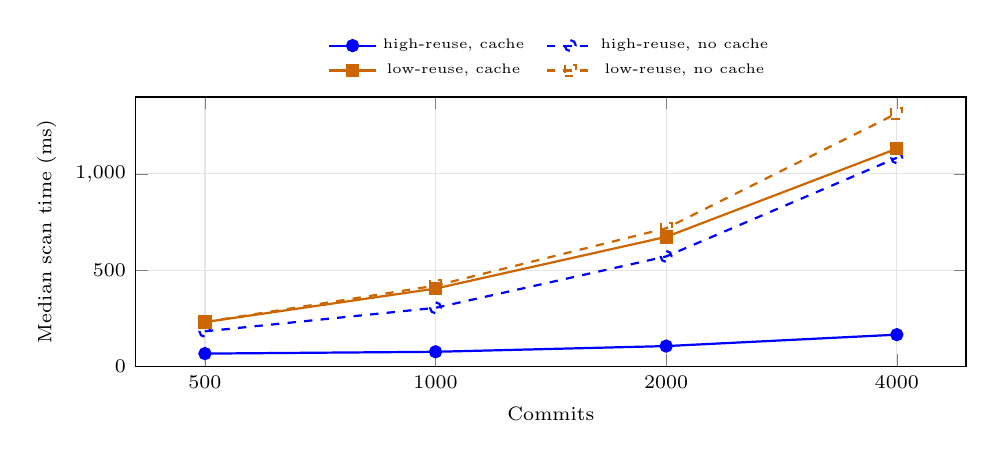
\begin{tikzpicture}
\begin{axis}[
  width=\columnwidth, height=50mm,
  xlabel={Commits}, ylabel={Median scan time (ms)},
  xmode=log, log basis x=2, xtick={500,1000,2000,4000},
  xticklabels={500,1000,2000,4000},
  ymin=0, ymax=1400,
  legend columns=2,
  legend style={font=\tiny,at={(0.5,1.03)},anchor=south,draw=none,/tikz/every even column/.append style={column sep=2mm}},
  tick label style={font=\scriptsize}, label style={font=\scriptsize},
  grid=major, grid style={gray!20}]
\addplot[mark=*,thick,blue] coordinates {(500,65.5) (1000,74.9) (2000,104.6) (4000,164)};
\addlegendentry{high-reuse, cache}
\addplot[mark=o,thick,blue,dashed] coordinates {(500,181.3) (1000,303.6) (2000,570.8) (4000,1084)};
\addlegendentry{high-reuse, no cache}
\addplot[mark=square*,thick,orange!80!black] coordinates {(500,229.4) (1000,403.7) (2000,672.6) (4000,1131.3)};
\addlegendentry{low-reuse, cache}
\addplot[mark=square,thick,orange!80!black,dashed] coordinates {(500,230) (1000,419.1) (2000,717.4) (4000,1314.8)};
\addlegendentry{low-reuse, no cache}
\end{axis}
\end{tikzpicture}
\caption{Median scan time against history length (data of Table~\ref{tab:memo}, E1). In the
high-reuse profile the cached scan grows slowly because the number of unique blobs stays at 150.}
\label{fig:memo}
\end{figure}

In the high-reuse profile, the number of blobs on which detection runs stays at 150 while the file
versions seen grow linearly with history, and the ratio of medians rises from 2.77$\times$ at 500
commits to 6.61$\times$ at 4{,}000 commits. In the low-reuse profile there is little to reuse and
the two modes take similar time (1.00$\times$ to 1.16$\times$): memoisation pays off in
proportion to blob reuse (reverts, copies, branches, generated files) and does nothing for
histories in which every change is unique. Even without the cache, the changed-files walk reads
far fewer file versions than a snapshot-per-commit scanner would (``Snapshot file versions'', a
count obtained by summing \code{git ls-tree -r} entries over all commits; it is not a timing).
These are single-machine timings of synthetic repositories and are not a prediction for any
particular real repository.

\subsection{Entropy calibration (E1)}
\emph{Command.} \code{npx tsx bench/entropy-calibration.ts 10000}, run on 2026-10-20 on E1 with
thresholds hex 3.0, base64 4.5, $n_{\min}=20$, $\lambda=0.85$. Each cell of
Table~\ref{tab:entropy} is the share of 10{,}000 seeded random strings (seed 2026) that
\emph{fail} the entropy check and would be missed. Length normalisation reduces the miss rate for
24-character alphanumeric strings from 95.21\% to 1.67\%, while the ordinary identifiers tested
(e.g.\ \code{getUserAccountSettingsForTenant}, $H=3.741$ against $T_{\text{eff}}=4.211$) are still
rejected. One tested string, the alphabet \code{abcdefghijklmnopqrstuvwxyz} ($H=4.700$), passes the
check, which illustrates why entropy is used only after a secret-like key name has been matched.

\begin{table}[t]
\centering
\caption{Share of Random Strings Missed by the Entropy Check (E1, $10^4$ Strings per Cell). N = Length-Normalised (Shipped), F = Fixed Threshold.}
\label{tab:entropy}
\footnotesize
\setlength{\tabcolsep}{2.2pt}
\begin{tabular}{@{}llrrrrrrrr@{}}
\toprule
Charset & & 16 & 20 & 24 & 28 & 32 & 40 & 48 & 64 \\
\midrule
\multirow{2}{*}{alnum} & N & 25.41 & 1.15 & 1.67 & 1.71 & 2.02 & 2.56 & 0.04 & 0.00 \\
 & F & 100.0 & 100.0 & 95.21 & 72.71 & 33.25 & 2.56 & 0.04 & 0.00 \\
\multirow{2}{*}{base64} & N & 23.80 & 1.11 & 1.43 & 1.48 & 1.58 & 1.83 & 0.04 & 0.00 \\
 & F & 100.0 & 100.0 & 94.65 & 70.57 & 29.92 & 1.83 & 0.04 & 0.00 \\
\multirow{2}{*}{hex} & N & 14.77 & 2.94 & 0.55 & 0.11 & 0.00 & 0.00 & 0.00 & 0.00 \\
 & F & 14.77 & 2.94 & 0.55 & 0.11 & 0.00 & 0.00 & 0.00 & 0.00 \\
\bottomrule
\multicolumn{10}{@{}l}{\scriptsize Column headings are string lengths $n$; cells are percentages.}
\end{tabular}
\end{table}

% ---------------------------------------------------------------------------------------------
\section{Discussion and Limitations}\label{sec:limits}

\emph{Tuning against the fixtures.} Five rule changes were made after scanning the fixtures or the
project's own repository, and are documented in \code{docs/RULES.md}: the length-normalised
threshold; normalising at $\max(n,n_{\min})$; requiring values under non-secret-like keys to be at
least $n_{\min}$ characters (which removed five false positives such as \code{DB\_HOST=localhost}
on \code{ci-configs}); excluding brackets from unquoted values; and suppressing values containing
a \code{\$\{\ldots\}} interpolation. These changes are the reason the fixture results in
Section~\ref{sec:eval} cannot be read as generalisation.

\emph{Known limitations} (\code{docs/ARCHITECTURE.md}, \code{docs/RULES.md}):
\begin{itemize}
\item Blobs or trees reachable only through a ref or tag that points directly at a blob or tree,
  rather than at a commit, are not scanned, since no commit exists to attribute them to.
\item At the default thresholds, roughly 1--3\% of random 20--40-character secrets with no
  recognisable format fail the entropy check (Table~\ref{tab:entropy}). This affects only
  entropy-layer candidates, never signature matches.
\item Presence is relative to \code{HEAD} (or the \code{--branch} tip); a secret that lives only on
  another branch is reported as \code{history-only}.
\item \code{dork} sees only what GitHub code search indexes: default branches, files under its size
  limit, non-fork repositories. Its findings are leads to confirm with \code{scan <repo-url>}.
\item Live verification covers long-term AWS keys with a paired secret and GitHub tokens only.
\item The signature set covers AWS, GitHub, Stripe, Slack and private keys; other providers are
  detected only through the generic key-name and entropy path.
\end{itemize}

% ---------------------------------------------------------------------------------------------
\section{Ethical Considerations and Responsible Use}\label{sec:ethics}

\tool{} is a defensive tool for repository owners, and several of its rules are enforced in code
rather than left to policy. Users must scan only repositories they own or are explicitly
authorised to scan; an authorisation notice is printed before any remote clone. Test repositories
use only fabricated, non-functional secrets, and a hygiene test fails if a token-shaped literal is
committed. Live verification requires two explicit flags, makes one read-only call per credential
to one of two allowlisted hosts, and discards account identifiers. The \code{dork} command refuses
to search outside the token owner's own account or administered organisation. There is no
telemetry: the only network access is a clone the user requests, opt-in verification, and
\code{dork} when run.

When a live credential is found, the documented procedure is to stop, record only the redacted
preview, path, commit and fingerprint, notify the owner privately, and let the owner rotate the
credential. A secret found in history must be treated as compromised and rotated first; rewriting
history with a tool such as \code{git filter-repo}~\cite{filterrepo} is secondary and does not undo
the exposure.

% ---------------------------------------------------------------------------------------------
\section{Conclusion}

\tool{} shows that a full-history, CI/CD-aware secret scanner can be built so that its safety
properties are structural rather than procedural: findings have no raw-secret field, the report
schema rejects unexpected fields, verification is opt-in and allowlisted, and the scanned
repository is treated as hostile input throughout. Blob-hash memoisation makes the cost of a
full-history walk depend on unique content rather than on commits~$\times$~files, and the measured
benchmark shows the effect growing with history length when content is reused. On the project's
own fixtures the tool detected all planted secrets, including merge-only and CI/CD literals that
the two compared tools missed in their default configurations; establishing real-world accuracy
requires an independent labelled corpus, which is the most important next step for this work.

\section*{Acknowledgment}
The authors thank Prof.\ Jyoti Yadav for guidance throughout this Ethical Hacking course project.

% ---------------------------------------------------------------------------------------------
\begin{thebibliography}{99}

\bibitem{cwe798}
MITRE, ``CWE-798: Use of hard-coded credentials,'' \emph{Common Weakness Enumeration}. [Online].
Available: \url{https://cwe.mitre.org/data/definitions/798.html}

\bibitem{meli2019}
M.~Meli, M.~R. McNiece, and B.~Reaves, ``How bad can it git? {C}haracterizing secret leakage in
public {GitHub} repositories,'' in \emph{Proc. Netw. Distrib. Syst. Secur. Symp. (NDSS)}, San Diego,
CA, USA, Feb. 2019.

\bibitem{filterrepo}
E.~Newren, ``git-filter-repo.'' [Online]. Available: \url{https://github.com/newren/git-filter-repo}

\bibitem{owaspcicd}
OWASP Foundation, ``OWASP top 10 {CI/CD} security risks.'' [Online]. Available:
\url{https://owasp.org/www-project-top-10-ci-cd-security-risks/}

\bibitem{codecov}
Codecov, ``Bash uploader security update,'' Apr. 2021. [Online]. Available:
\url{https://about.codecov.io/security-update/}

\bibitem{gitleaks}
Gitleaks, ``Gitleaks: Find secrets with Gitleaks.'' [Online]. Available:
\url{https://github.com/gitleaks/gitleaks}

\bibitem{trufflehog}
Truffle Security, ``TruffleHog.'' [Online]. Available:
\url{https://github.com/trufflesecurity/trufflehog}

\bibitem{sinha2015}
V.~S. Sinha, D.~Saha, P.~Dhoolia, R.~Padhye, and S.~Mani, ``Detecting and mitigating secret-key
leaks in source code repositories,'' in \emph{Proc. 12th IEEE/ACM Working Conf. Mining Softw.
Repositories (MSR)}, Florence, Italy, 2015, pp.~396--400.

\bibitem{secretbench}
S.~K. Basak, L.~Neil, B.~Reaves, and L.~Williams, ``{SecretBench}: A dataset of software secrets,''
in \emph{Proc. 20th IEEE/ACM Int. Conf. Mining Softw. Repositories (MSR)}, Melbourne, Australia,
2023, pp.~347--351.

\bibitem{basak2022}
S.~K. Basak, L.~Neil, B.~Reaves, and L.~Williams, ``What are the practices for secret management in
software artifacts?'' in \emph{Proc. IEEE Secure Develop. Conf. (SecDev)}, 2022.

\bibitem{ghsecretscanning}
GitHub, ``About secret scanning,'' \emph{GitHub Docs}. [Online]. Available:
\url{https://docs.github.com/en/code-security/secret-scanning}

\bibitem{shannon1948}
C.~E. Shannon, ``A mathematical theory of communication,'' \emph{Bell Syst. Tech. J.}, vol.~27,
no.~3, pp.~379--423, Jul. 1948.

\bibitem{gitlog}
Git Project, ``git-log documentation,'' \emph{Git Reference Manual}. [Online]. Available:
\url{https://git-scm.com/docs/git-log}

\bibitem{gitcatfile}
Git Project, ``git-cat-file documentation,'' \emph{Git Reference Manual}. [Online]. Available:
\url{https://git-scm.com/docs/git-cat-file}

\bibitem{clrs}
T.~H. Cormen, C.~E. Leiserson, R.~L. Rivest, and C.~Stein, \emph{Introduction to Algorithms},
4th~ed. Cambridge, MA, USA: MIT Press, 2022.

\bibitem{rfc4122}
P.~Leach, M.~Mealling, and R.~Salz, ``A universally unique identifier ({UUID}) {URN} namespace,''
IETF, RFC~4122, Jul. 2005.

\bibitem{awssts}
Amazon Web Services, ``GetCallerIdentity,'' \emph{AWS Security Token Service API Reference}.
[Online]. Available:
\url{https://docs.aws.amazon.com/STS/latest/APIReference/API_GetCallerIdentity.html}

\bibitem{awssigv4}
Amazon Web Services, ``AWS Signature Version 4 for API requests,'' \emph{IAM User Guide}.
[Online]. Available: \url{https://docs.aws.amazon.com/IAM/latest/UserGuide/reference_sigv.html}

\bibitem{ghusers}
GitHub, ``REST API endpoints for users,'' \emph{GitHub Docs}. [Online]. Available:
\url{https://docs.github.com/en/rest/users/users}

\bibitem{jsonschema}
JSON Schema, ``JSON Schema draft 2020-12.'' [Online]. Available:
\url{https://json-schema.org/draft/2020-12}

\bibitem{csp3}
W3C, ``Content Security Policy level 3,'' W3C Working Draft. [Online]. Available:
\url{https://www.w3.org/TR/CSP3/}

\bibitem{ghsearch}
GitHub, ``REST API endpoints for search,'' \emph{GitHub Docs}. [Online]. Available:
\url{https://docs.github.com/en/rest/search/search}

\bibitem{redos}
OWASP Foundation, ``Regular expression denial of service -- ReDoS.'' [Online]. Available:
\url{https://owasp.org/www-community/attacks/Regular_expression_Denial_of_Service_-_ReDoS}

\end{thebibliography}

\end{document}
